\documentclass{jarticle}
\usepackage[margin=20truemm]{geometry}
\usepackage{setspace}
\usepackage[mathlines]{lineno} %% <- remove [mathlines] to omit equation line numbers
\usepackage{amsmath}
\usepackage[dvipdfmx]{graphicx}

\usepackage{mathtools}

\usepackage{listings,jvlisting} 
\usepackage{etoolbox} %% <- for \pretocmd, \apptocmd and \patchcmd

\doublespacing


%% Patch 'normal' math environments:
\newcommand*\linenomathpatch[1]{%
  \cspreto{#1}{\linenomath}%
  \cspreto{#1*}{\linenomath}%
  \csappto{end#1}{\endlinenomath}%
  \csappto{end#1*}{\endlinenomath}%
}
%% Patch AMS math environments:
\newcommand*\linenomathpatchAMS[1]{%
  \cspreto{#1}{\linenomathAMS}%
  \cspreto{#1*}{\linenomathAMS}%
  \csappto{end#1}{\endlinenomath}%
  \csappto{end#1*}{\endlinenomath}%
}

%% Definition of \linenomathAMS depends on whether the mathlines option is provided
\expandafter\ifx\linenomath\linenomathWithnumbers
  \let\linenomathAMS\linenomathWithnumbers
  %% The following line gets rid of an extra line numbers at the bottom:
  \patchcmd\linenomathAMS{\advance\postdisplaypenalty\linenopenalty}{}{}{}
\else
  \let\linenomathAMS\linenomathNonumbers
\fi

\linenomathpatch{equation}
\linenomathpatchAMS{gather}
\linenomathpatchAMS{multline}
\linenomathpatchAMS{align}
\linenomathpatchAMS{alignat}
\linenomathpatchAMS{flalign}

\linenumbers
\title{My Document}
\author{Anonymous Anteater}

\begin{document}
\maketitle
\begin{abstract}

\end{abstract}
\section{Introduction}



\subsection{Background}
In astrophysics and astronomy, to numerically calculate the dynamical 
evolution of N particles interacting gravitationally, N-body simulations 
are required. Figure 1 shows the equation for interparticle interactions 
in N-body simulations. If the equation is naively computed, the time
complexity of calculation of interparticle interactions is 
\begin{math}O(N^2) \end{math}, where 
N is the number of particles. Therefore, parallelization is required to
speed up numerical simulations. To write a parallelized code for a 
numerical simulation, a user needs to understand the architecture of 
computer systems in  detail. If a parallelized code is automatically
generated by only describing the formulas and data of the numerical
simulation, the above problems are solved. To realize the parallelization,
we will develop Domain Specific Language  DSL \rparen, which is a 
programming language specialized to a domain, for example, SQL and HTML.


\subsection{parallelization}
SIMD is one of the categories in Flynn's taxonomy 1, related to computer arithmetic
 processing. Using SIMD, arithmetic operations can be applied simultaneously to
multiple data. In this paper, we compute and parallelize multiple particles. For example, 
as shown in Figure 1, the computation of acceleration for different particles is independent
of each other, allowing the process to be parallelized. As a result, for instance Assuming 
that the variables for particles are double-precision floating-point numbers, we can execute 
an operation on four elements simultaneously using the AVX2 instruction, it is possible to 
perform operations on four elements. Therefore, compared to non-parallelized code, there is
a potential to accelerate the computation by four times. We will describe the design of a 
DSL in the next section to generate such parallelized code from the formulation of particle-particle interactions.

\subsection{Overview of DSL}
私たちはPykerというDSLを作成しました。この言語の処理系は粒子相互作用の式を記述したコードを読み込み、
その計算を高速化するC++言語のコードを生成することが出来る。この言語は変数を定義と相互作用の式を記述できる。
変数を定義する部分では、粒子の質量や位置、結果を保存する変数、それ以外に必要となる変数を定義できる。
式の部分では、相互作用の式に必要な四則演算やsqrt,べき乗,ベクトルの内積を計算できるようにした。
この記述からkernel関数を生成し、それを呼び出して使う。



\section{Construction}
私たちはDSLの実装にPythonの代数計算ライブラリのSympyを使った。
Sympyでは、数式をシンボルと演算子を用いて構文木として扱うことが出来る。
そしてその構文木から実行可能なコードを生成するモジュールがある。このDSLでは、それらの機能を用いて数式を読み込み、
並列に実行できるコードを生成する。並列化には、Advanced Vector Extensions 2(AVX2)という命令セットを用いた。AVX2とは、
インテル社のCPUに実装された拡張命令セットの一つである。次のセクションでは、どのようにAVX2で並列化を行うかを説明する。

\subsection{AVX2 for parallelization}

SIMDを行うには通常の計算と同じように、まずメモリからデータをloadし、そのデータをもとに計算し、結果をstoreする。
しかし、SIMDの場合は、SIMD用のレジスタを使って計算をするためloadや計算、storeの仕方が違う.loadをするとき,
SIMD用のレジスタに同じ命令を行う複数の要素を格納する。そしてそれを使って同時に計算し、計算結果をそれぞれstoreする。

 例えば、倍精度小数の配列x,yの要素を計算するC=X + Yのような計算を考えるとき,AVX2を使用してSIMDを行う場合レジスタは
256ビットのレジスタなので、xとyの要素をそれぞれ4つずつloadする。そしてそれを同時に足し、結果を格納する配列Cにstoreする。
SIMDレジスタにloadをするとき、1次元配列なら連続するメモリをアクセスすればいいが、Figure a.に示すArray of Structures\lparen AoS \rparen
のデータ構造の場合、要素ごとにロードしてこなくてはいけない。

 例えば、粒子の3次元の座標を倍精度小数でpos [n] \lbrack 3\rbrack 
 \lparen nは粒子の総数とし、pos \lbrack i \rbrack \lbrack 0\rbrack ,pos\lbrack i \rbrack \lbrack 1 \rbrack, pos \lbrack i \rbrack \lbrack 2 \rbrack をそれぞれi番目の粒子のx座標,y座標,z座標 \rparen
  とするとき、粒子i, jのx座標の差を求めるとき、dx = pos \lbrack i \rbrack \lbrack 0 \rbrack - pos\lbrack j \rbrack \lbrack 0 \rbrack のようになるが,
これをSIMDで並列化するとき、
\begin{lstlisting}[frame=single]
dx0 = pos[i][0] - pos[j][0]
dx1 = pos[i + 1][0] - pos[j][0]
dx2 = pos[i + 2][0] - pos[j][0]
dx3 = pos[i + 3][0] - pos[j][0]
\end{lstlisting}
  
としたいので、\lparen pos\lbrack  j\rbrack \lbrack  0\rbrack , pos\lbrack  j\rbrack \lbrack  0\rbrack , pos\lbrack  j\rbrack \lbrack  0\rbrack , pos\lbrack  j\rbrack \lbrack  0\rparen, \lparen
,\lparen dx0,dx1,dx2,dx3 \rparen とそれぞれパックして、同時に引き算を行う。しかし、SIMDレジスタにデータを一度にそれぞれ乗せなくてはいけないので、
gather命令を使い粒子iのデータをloadする。gather命令とは、アドレスを指定してメモリアドレス上の連続していないデータ要素を読み込むのに使用する。
gather命令の説明を図xに示す。このようにloadしたデータをSIMDの命令を実行し同時に計算する。


計算結果をstoreする際もアドレスが連続していない場合がある。その時は、scatter命令と呼ばれるgather命令と対象になる命令があるが、
AVX2にはサポートされていないため、それぞれポインタを使ってデータをstoreする。このようにしてSIMDによる並列化をする。

また、これらの命令はinstrinsincs関数を使うことでC,C++などの**high-level programming languageにおいて**明示的に扱える。
C,C++においてinstrinsincs関数を扱うには、言語標準で使用できるimmintrin.hというファイルをインクルードする。
そしてデータはtemplate.cppをx座標の差を計算するC++のコードを例として示す。Pykerは記述された数式をtemplate.cpp
のようにSIMD命令を実行できるようなC++のコードを生成する。次のセクションでは、Pykerの説明する。


\subsection{Pyker}
このDSLでは、変数の定義と相互作用の式の定義の2つを記述しそれをコンパイルすることでコードを生成する。最初に変数定義について説明する。

このDSLでは、変数にはclassがあり、EPI,EPJ,FORCE,その他と分かれる。EPIは相互作用を受ける粒子を示し、EPJが相互作用を与える粒子になる。
FORCEは相互作用の計算結果を保持し、そのほかの変数はソフトニングパラメータ等である。これらの変数を使って計算をするには、
C++では、template.cppのようになる。


\begin{lstlisting}[frame=single, caption=template.cpp, language=c++]
  int kernel(EPI epi, EPJ epj, FORCE force, double eps2, int n){
    // (1).preprocess
    for(int i = 0;i < n;i += 1) {
      // (2).load EPI 
      // (3).Initialization of tmporary force
      for(int j = 0;j < n;j += 1) {
          // (4). calculate interparticle interactions
      }
      // (5). Store calculation result in the FORCE
    }
  
  }
  \end{lstlisting}

  (1)では、計算に必要な変数の定義などの前準備。(2)では、EPIの変数をロードする。(3)では、相互作用の計算結果を一時的に保持する変数を初期化。
  (4)では、相互作用の計算を行い、結果をforceの一次変数に保存。(5)で,FORCEの変数に結果をstoreする。

  このコードを生成するためには、変数の定義では、変数のclassと、型、次元の情報がそれぞれ必要になる。そのためpykerでは、変数の定義を正規表現で表すと以下のようになる。
  \begin{lstlisting}
  ((EPI|EPJ|FORCE).(\w+))? (vec3<)?(F64)>? \w+
  \end{lstlisting}
  
  1列目はclassであれば、classの名前とそのメンバ変数名を書く。2列目はベクトルの次元があれば、明示的に書き、
  型は'F64'と書き、64bit浮動小数を表す。3列目では、pykg上で扱う変数の名前になる。例えば、”EPI.pos vec3<F64> xi”は、EPIのposというメンバ変数で、
  3次元の64bit浮動小数型のxiという変数名となる。
  
  相互作用の式の定義は、定義した変数を使って、FORCEの変数に結果をアキュムレートしていくように記述する。
  数式の記述に必要な一次変数はそれまでに定義された変数を用いてを新たに定義できる。使用できる演算は、四則演算とsqrtとべき乗を表す'**'を使うことが出来る。
  結果はFORCEの変数に'='でstoreすることを表す。
  
  例えば、Figure 1の重力相互作用の式を計算するコードを生成する場合、このDSLで記述するとtemplate.pykerとなる。

\begin{lstlisting}[frame=single, caption=hoge, label=fuga]
  EPI.pos vec3<F64> xi
  EPJ.pos vec3<F64> xj
  EPJ.m F64 mass
  FORCE.acc vec3<F64> ai
  F64 eps2
  F64 g
  dr = xj - xi
  ai = g * mass *  dr / sqrt(dr ** 2 + eps2) ** 3
\end{lstlisting}

次のセクションでは、どのようにして、このコードから目標のコードを生成するかを説明する。


\subsection{Implementation}
コードを生成する流れは以下のflowchartに示す。Parseでは、DSLのコードから定義された変数の情報を変数名をkeyに持つハッシュに変換する。
数式は、Sympy形式の構文木に変換し、そのリストを取得する。次に構文木に変換した数式に対してCommon subexpression elimination(CSE)を行う。
CSEとは、数式に含まれる共通部分式をあらかじめ計算し、その計算結果を使って数式を計算することによって演算回数を減らすことである。type inferenceでは、
数式の一次変数の型推論を行う。その後数式をSIMD演算に合わせるため構文木をすべて二分木にする。最後に以上の処理を行った構文木を辿り、相互作用の計算を行うコードを生成する。
以下は、ParseからCSE,type inference, convert to binary tree, Codegenerateの順にどのように実装を行ったかを説明していく。
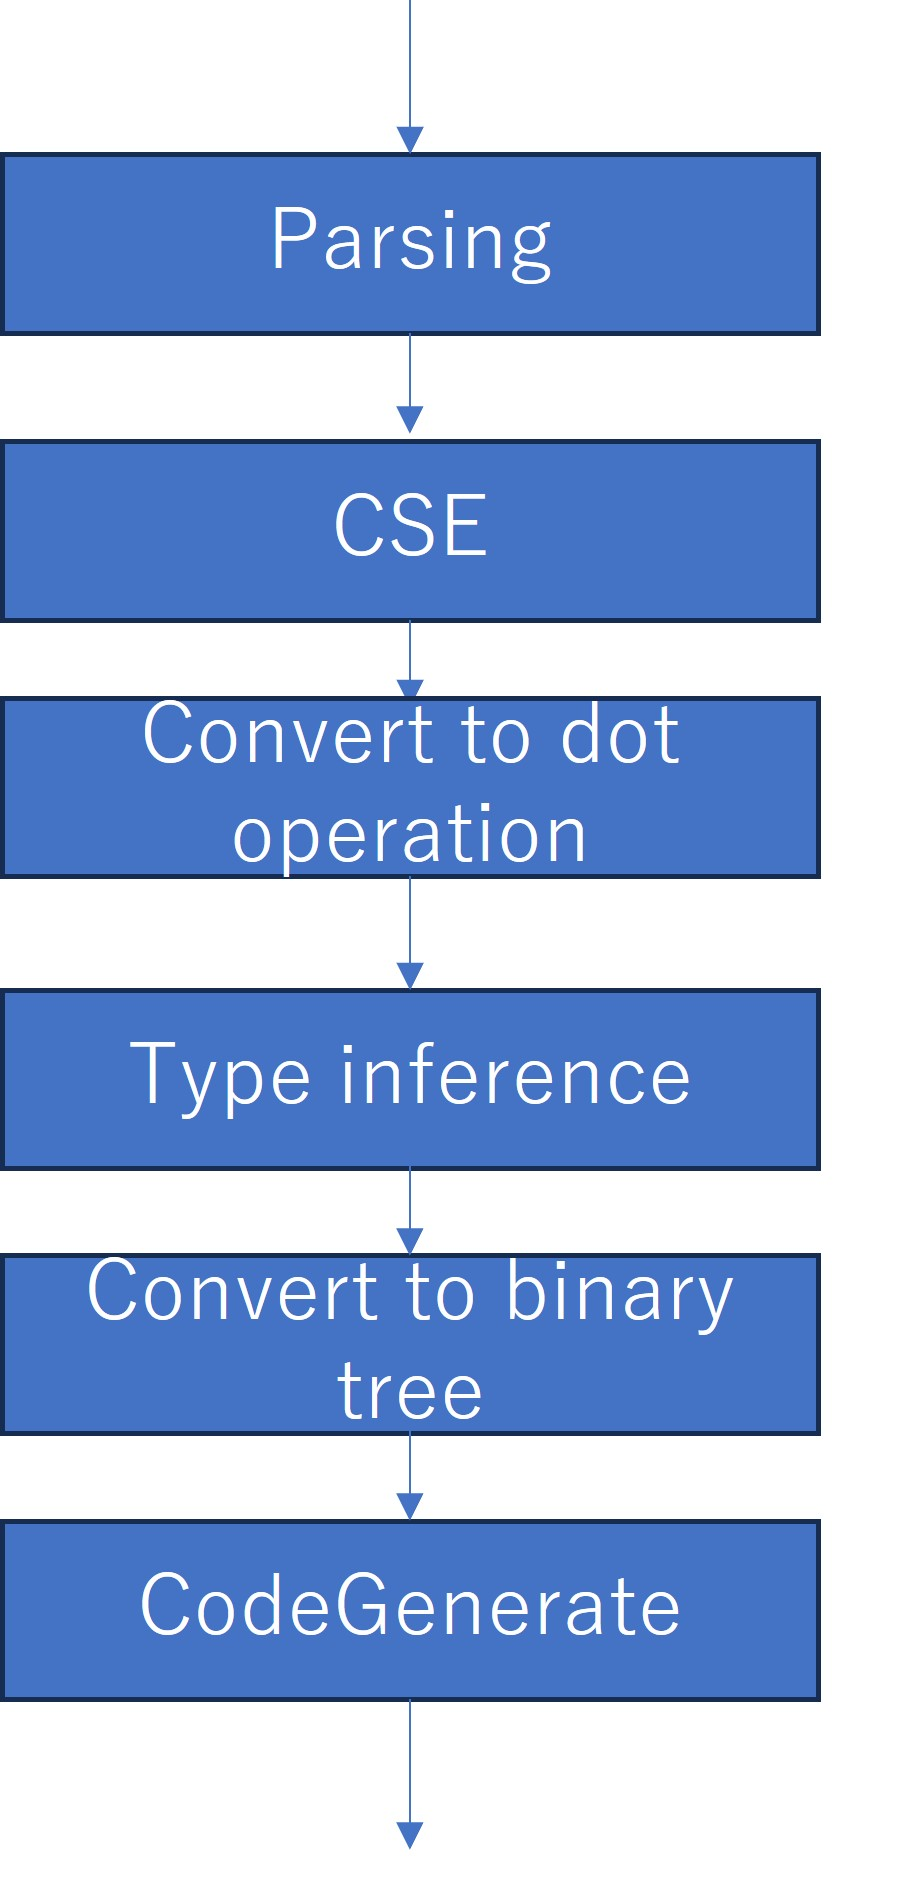
\includegraphics[width=100mm]{flowchartver3.jpg}


\subsubsection{Parsing}
Parseでは、変数定義と数式で処理を分ける。変数定義では,class, ベクトル、型、変数名を持つ自作したVarというクラスのオブジェクトをそれぞれ生成する。
そのオブジェクトとkeyを変数名に持つハッシュを作る(name\_variable\_map)。数式はSympyのライブラリにあるメソッドのsympify()を使い、
文字列として読み込んだコードを数式の構文木に変換し、それらの構文木のリスト(expr\_list)を取得する。次にCSEを行う。


\subsubsection{CSE}

CSEとは数式にある共通する部分式を先に計算し、その結果を使うことで演算回数を減らすこと。これにはsympyにあるcse()という関数に数式を渡して行う。これにより新たに部分式の数式が生成されて、その部分式の結果を使った計算式に変換される。


\subsubsection{translate to dot method}
このDSLでは、ベクトル同士の積を内積として扱う。そのために、構文木をたどっていき該当する部分式を見つけてそこを置き換えて木を再構築する。
sympyの構文木の構造は演算子が親となり、その子としてほかの演算子やシンボルがある。例えば、x,y,z を変数としてx + y * z は図1のような構文木になる。
しかしこの要素らがベクトルであるかがsympyが知らないため例えば、v1,v2をベクトル、v3をスカラーととこのDSL上で定義されていたとすると、(v1 * v2) * v3
は一つのMulが親となり、v1,v2,v3が子となる構文木になる。そのため、完全二分木にする際、どこが内積に該当するのかわからない。なので内積をdot関数に置き換える。
sympyにはFunctionCallというclassがあり、独自に定義した関数を構文木に組み込むことが出来る。そのため、構文木をたどり該当する部分木をFunctionCallでdot関数に置き換えていく。
その構文木をたどる際、ノードが部分式の場合、その部分式が返すのがベクトルかどうかわからない。
そのためkeyにノードを持ちvalueにベクトルかスカラーかの情報を持つhash(arg\_ret\_map)を作り、それを使って判定する。そして、dotに置き換え更新した部分式はarg\_ret\_mapにその都度更新する。
こうしてdot演算に置き換え再構築した構文木のリストを次の処理に渡す。

\subsubsection{type inference}
一時変数は数式の結果を一時的に保存する。その一時変数の型やベクトルを判断するには、数式の結果がどんな型なのかどんなvecなのかでわかる。
またこのDSLでは型は倍精度少数しか実装していないので、ベクトルかどうかだけが分かればいい。そのため、CSEのセクションで説明したarg\_ret\_mapを使う。

\subsubsection{convert to binary trees}
simd演算はinstrcin関数で行う際2項演算なので引数が2つの関数を使って数式を計算するコードにしなければならない。そのため、数式の構文木を完全二分木である必要がある。
しかし、sympyの数式の構文木では演算の順序を考えなくてよい場合、一つの演算子を親としてその項をまとめる。そのため、子を3つ以上持つような演算子のノードでは、
その演算子で二分木に変換する。例を図1に示す。このときsympyが自動で簡約化して二分木をまとめてしまわないように、演算子に置き換えるときに演算子の関数を使い、
オプションでevaluate=Falseにする。例えばa * b * c はMul(a, Mul(b, c, evaluate=False), evaluate=False)となる。



\subsubsection{code generation of SIMD}
CodeGenでは、c++で実行可能な関数のコードを生成する。生成するコードの疑似コードをtemplate.cppに示す。

\begin{lstlisting}[frame=single, caption=template.cpp]
  //(1) include part
  #include<math>
  #include<immintrin.h>
  int kernel( (2) double xi[][3], double xj[][3], double eps2, double ai[][3], ...) {
    //(3) decleare tmp variable
    int i;
    int j;
    __m256d xi_tmp_v0;
    __m256d xi_tmp_v1;  
    __m256d xi_tmp_v2;
    __m256d eps2_tmp;
    // ... 
    // ... 
    // ... 
    //(4) def not class variables
    eps2_tmp = _mm256_set1_pd(eps2);
    // ... 
    // ... 
    // ... 
    
    // (5) loop increment
    for(i = 0;i < (n);i += 4) {
      // (6) Load EPI variable part
      int index_gather_0[4] = {0, 3, 6, 9};
      __m128i vindex_gather_0 = _mm_load_si128((const __m128i*)index_gather_0);    
      xi_tmp_v0 = _mm256_i32gather_pd(&xi[i][0], vindex_gather_0, 8);
      // ... 
      // ... 
      // ... 
      // (7) initialize result temporary variable
      ai_tmp_v0 = _mm256_set1_pd(0.0);
      ai_tmp_v1 = _mm256_set1_pd(0.0);
      ai_tmp_v2 = _mm256_set1_pd(0.0);
  
      for(j = 0;j < (n);j += 1) {
        // (8) Load EPJ variable part
           xj_tmp_v0 = _mm256_set1_pd(xj[j][0]);
           xj_tmp_v1 = _mm256_set1_pd(xj[j][1]);
           xj_tmp_v2 = _mm256_set1_pd(xj[j][2]);
          // ... 
          // ... 
          // ... 
           
  
        // (9) calculate interparticle
      }
  
      // (10) Store result part
  
    }
    return 0;
  }
  \end{lstlisting}


コード生成の際に必要な要素をtemplate.cppに書かれた(1), (2),(3)の順に説明する。それぞれは(1)インクルード文の挿入、(2)関数の引数の定義、(3)相互作用の計算に必要な一時変数,(4)EPI,EPJ,FORCEでない変数の定義、(5)ループのインクリメント幅、(6)EPIの変数をloadする部分、(7)結果を一時的に保持する変数の初期化、(8) EPJの変数をロードする部分、(9)実際に計算する内容、(10)SIMDのstore部分である。またDSL上で定義したEPI,EPJ,FORCEの変数は、ソースコード上では単なる変数として扱われる。

(1)では、SIMD演算などで必要となるインクルード文を挿入する。math.hは、SIMD化しない場合に、sqrt()を実行するために、immintrin.hでは、SIMD演算のための関数を呼び出すために必要となる.

(2)では、DSLのコードで変数定義されていた変数を引数とする。そのために変数をすべてみて、DSLのコードで変数定義されていれば引数に追加する。

(3)Sympyでは、変数の定義をVariableというクラスのオブジェクトをDeclarationというクラスのコンストラクタに渡して生成したオブジェクトで表す。

一時変数の名前はベクトルであれば、(DSL上で記述した名前)\_tmp\_v{i}(iは次元数に合わせて0インデックスで定義), スカラーであれば、(DSL上で記述した名前) \_tmpとする。変数の型は今回は倍精度少数だけなので、\_\_m256dにする。\_\_m256dはAVX2の256bitのレジスタで要素が倍精度少数をセットできる型である.

(4)では、classでない変数の定義では、定義とともにその変数の値を並列する数分初期化する。それには,\_mm256\_set1\_pd()という関数を使う。この関数は引数で与えられた倍精度少数の値を\_\_m256dに4つセットする関数で、eps2\_tmpのデータ構造は(eps2, eps2, eps2, eps2)のようになっている。これとループで使用するインデックスである,iとjを定義する.

(5)では、並列数分だけインクリメントするようにする。今回は倍精度少数しか実装していないので並列数は常に4にする.

(6)では、EPIの変数のloadを行う。loadには、AVX2 for Parallelizationのセクションで説明したようにgather命令を使用する。gather命令は、
(6)に書かれている3行のコードはgather命令によるloadの一連の流れである。index\_gather\_0[]は\& xi[i][0]から何個分のメモリにあるかを示している。\&xi[i][0]から\&xi[i + 1][0]
はdouble型の変数の3つ分先のメモリアドレスになる。\&xi[i + 2][0]も同様になるのでindex\_gather\_0[]には、{0, 3, 6,9}となる。vindex\_gather\_0はindex\_gather\_0を128ビットレジスタに乗せていて、
これで\_mm256\_i32gather\_pdを使うことが出来る。\_mm256\_i32gather\_pdの第3引数の8は、要素が何バイトであるかを表し、double型なので8byteとしている。これにより、
\&xi[i][0],\&xi[i + 1][0],\&xi[i + 2][0],\&xi[i + 3][0]をロードする。またEPIの要素がスカラーであれば、\_mm256\_load\_pd(\&m[i])という関数を使い、連続するm[i],m[i+1],m[i+2],m[i+3]を256ビットのレジスタにloadする。
これをEPIの変数すべてに行う。
% - このセクションでは、実行可能なコードを生成する。
% - コードを生成するには、Codegenというモジュールを使う。
%     - このモジュールはsympyの数式から実行可能なコードを生成するモジュールである。
%     - このDSLでは、関数を作成するのに**FunctionDefinition**というクラスのオブジェクトを生成し、それを出力する。FunctionDefinitionでは、関数のsympyで定義した計算内容とFunctionPrototypeというクラスのオブジェクトを引数としてfrom\_FunctionPrototypeというFunctionDefinitionのメンバ関数によってFunctionDefinitionのオブジェクトを生成する。そして最後に、必要なinclude文を追加し,hppのファイルとして出力する。
%     - FunctionDefinitionの生成
%         - FunctionPrototypeと計算内容が必要
%     - FunctionPrototypeの生成
%         - 関数の引数と戻り値と名前が必要
%         - 引数は、DSL上で定義した変数
%         - 戻り値は、今回はintで0を返すようにする
%         - 名前はkernelとする
%     - 計算内容
%         - template.cppの(1)~(5)
%         - (1)は計算に必要な一時変数の定義する文を作成
%         - (2)でgather命令を用いたload。ここでは、FunctionCall()を使ってintrinsics関数のgather命令に対応する関数を呼び、それを代入する文を作成する
%         - (3)で計算結果を保持する一時変数を初期化
%         - (4)数式のリストから演算子をSIMD命令に置き換えていく。
%         - またここで、引き算、割り算、sqrt、べき乗は単純に置き換えられない。
%             - 引き算の場合は、sympyは構文木にすると引き算をx + ((-1) * y)のようになっていて演算子の引き算がノードとなっていない。そのため、今探索しているノードがAddだった場合、子に-1がかかっている要素があれば、引き算のSIMD命令に置き換える。
%             - 割り算の場合は、引き算の場合と同様に、構文木に割り算がないため、\begin{math}x / y \end{math} を \begin{math}
%               x * (y ^(-1))
%             \end{math}と表現されているので、探索しているノードが掛け算のとき、子に-1乗されてるノードがあれば割り算のSIMD命令にする。
%             - sqrtの場合は、例えばsqrt(x)は構文木上では、\begin{math}x^(1/2) \end{math}と表されているので、同様にべき乗の演算子Powのの時, expが1/2であれば、sqrtのSIMD命令に置き換える。
%         - 計算に必要な一時変数
%     - CodeBlockというクラスのオブジェクトを生成する
%     - 
%     - forループ,load,結果を一時保存する初期化、
%     - Loadパート
%     - そもそも
\begin{table}
  \centering % 表を中央揃えにする
  \caption{サンプル表} % 表のタイトル
  \label{tab:sampleTable}
  \begin{tabular}{ccc} % ここで列の数とテキストの配置を指定
  \toprule
  N & Pyker & PIKG \\
  \midrule
  50000 & 5.282461100 & 4.059262 \\
  25000 & 1.322715200 & 1.008046 \\
  10000 & 0.213696 & 0.161884 \\
  1000 & 0.002116 & 0.001713 \\
\bottomrule
\end{tabular}
\end{table}
\begin{table}[ht]
  \centering % 表を中央揃えにする
  \caption{サンプル表} % 表のタイトル
  \label{tab:sampleTable}
  \begin{tabular}{ccc} % ここで列の数とテキストの配置を指定
  \toprule
  項目 & 値 & 単位 \\
  \midrule
  項目1 & 100 & kg \\
  項目2 & 200 & g \\
  項目3 & 300 & mg \\
\bottomrule
\end{tabular}
\end{table}


\begin{table}[ht]
  \centering % 表を中央揃えにする
  \caption{サンプル表} % 表のタイトル
  \label{tab:sampleTable}
  \begin{tabular}{ccc} % ここで列の数とテキストの配置を指定
  \toprule
  N & Pyker & PIKG \\
  \midrule
  50000 & 24.755255 & 22.767920 \\
  25000 & 6.136025 & 5.740028 \\
  10000 & 1.044833 & 0.901585\\
  1000 & 0.010176 & 0.009109 \\
\bottomrule
\end{tabular}
\end{table}

\begin{table}[ht]
  \centering % 表を中央揃えにする
  \caption{サンプル表} % 表のタイトル
  \label{tab:sampleTable}
  \begin{tabular}{ccc} % ここで列の数とテキストの配置を指定
  \toprule
  N & Pyker & PIKG \\
  \midrule
  50000 & 13.796789& 10.794405\\
  25000 & 3.472925 & 2.693424\\
  10000 & 0.557972 & 0.424820\\
  1000 & 0.005405& 0.004240\\
\bottomrule
\end{tabular}
\end{table}



\begin{table}[ht]
  \centering % 表を中央揃えにする
  \caption{サンプル表} % 表のタイトル
  \label{tab:sampleTable}
  \begin{tabular}{ccc} % ここで列の数とテキストの配置を指定
  \toprule
  N & Pyker & PIKG \\
  \midrule
  50000 & 2.476695 & 2.439798\\
  25000 & 0.617220 & 0.598798\\
  10000 & 0.094859 & 0.094860\\
  1000 & 0.000939& 0.000988\\
\bottomrule
\end{tabular}
\end{table}


\begin{table}[ht]
  \centering % 表を中央揃えにする
  \caption{サンプル表} % 表のタイトル
  \label{tab:sampleTable}
  \begin{tabular}{ccc} % ここで列の数とテキストの配置を指定
  \toprule
  N & Pyker & PIKG \\
  \midrule
  50000 & 2.153937 & 2.194700\\
  25000 &0.542478 & 0.554280\\
  10000 & 0.085537 &0.087284\\
  1000 & 0.000869&0.000874\\
\bottomrule
\end{tabular}
\end{table}

\begin{table}[ht]
  \centering % 表を中央揃えにする
  \caption{サンプル表} % 表のタイトル
  \label{tab:sampleTable}
  \begin{tabular}{ccc} % ここで列の数とテキストの配置を指定
  \toprule
  N & Pyker & PIKG \\
  \midrule
  50000 & 15.103493& 9.904044\\
  25000 &3.736596 & 2.480025\\
  10000 &0.543367 &0.398513\\
  1000 & 0.005392&0.003911\\
\bottomrule
\end{tabular}
\end{table} 

\end{document}


